\documentclass[a4paper]{article}

\usepackage[14pt]{extsizes}
\usepackage[T2A]{fontenc}
\usepackage[russian]{babel}

\usepackage[left=20mm, top=15mm, right=15mm, bottom=20mm]{geometry}
\usepackage{listings}
\usepackage{xcolor}
\usepackage{tikz}
\usetikzlibrary{shapes.geometric, arrows.meta, positioning, calc, arrows, shapes.misc}
\usepackage{graphicx}
\usepackage{amsmath, amssymb} % For equations
\usepackage{booktabs} % For better tables
\usepackage{pgfplots} % For plotting graphs
\usepackage{caption} % For captioning tables and figures
\usepackage{float} % For precise float placement (images, tables)
\usepackage[hidelinks]{hyperref} % For table of contents to be clickable
\usepackage{bookmark}
\usepackage{multirow}
\usepackage{array}
\usepackage{cancel}
\usepackage{placeins}
\usepackage{enumitem}
\pgfplotsset{compat=1.17}
\usepackage{circuitikz}
\usetikzlibrary{decorations.markings} % For custom arrow positioning

% -----------------------------------------------------

\newcommand{\labtitle}[9]{
	\begin{center}
		\vspace*{-1.8cm}
		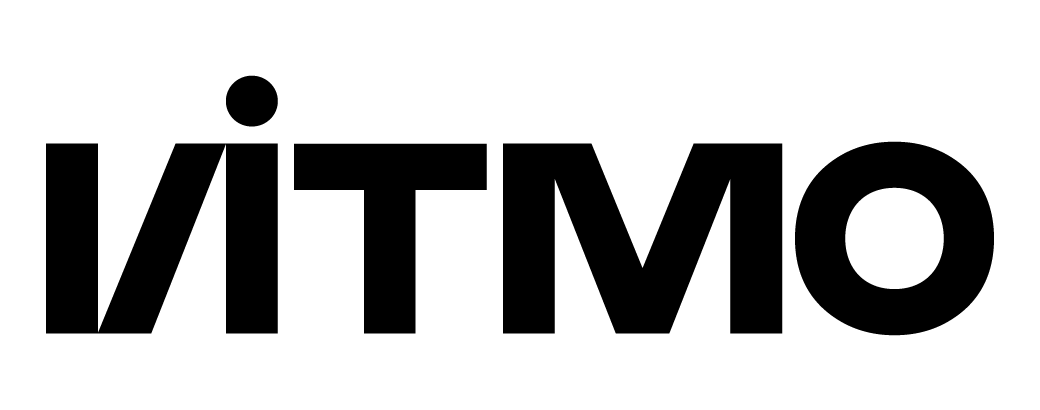
\includegraphics[width=0.26\textwidth]{../common/itmo-logo.png}\\
		\vspace{2.4cm}
		\textbf{\Large Основы электротехники}\\[1.2cm]
		\textbf{\Large Отчёт по лабораторной работе №#1}\\[0.7cm]
		\textbf{\Large #2}\\[3cm]

		\textbf{\Large Группа \textcolor{red}{\textit{P#3}}}\\[0.2cm]
		\textbf{\Large Вариант \textcolor{red}{\textit{#4}}}\\[3cm]

		\begin{flushleft}
			\textbf{\large Выполнил: \textcolor{red}{\textit{#5}}}\\[0.5cm]
			\textbf{\large Дата сдачи отчёта: \textcolor{red}{#6}}\\[0.5cm]
			\textbf{\large Дата защиты: \textcolor{red}{#7}}\\[0.5cm]
			\textbf{\large Контрольный срок защиты: \uline{#8}}\\[0.5cm]
			\textbf{\large Количество баллов: \uline{#9}}\\[2cm]
		\end{flushleft}
	\end{center}

	\vspace*{\fill}
	\begin{center}
		\textbf{\Large СПб -- 2024}
	\end{center}
	\vspace*{-1.8cm}
}

\newcommand{\hwtitle}[8]{
	\begin{center}
		\vspace*{-1.8cm}
		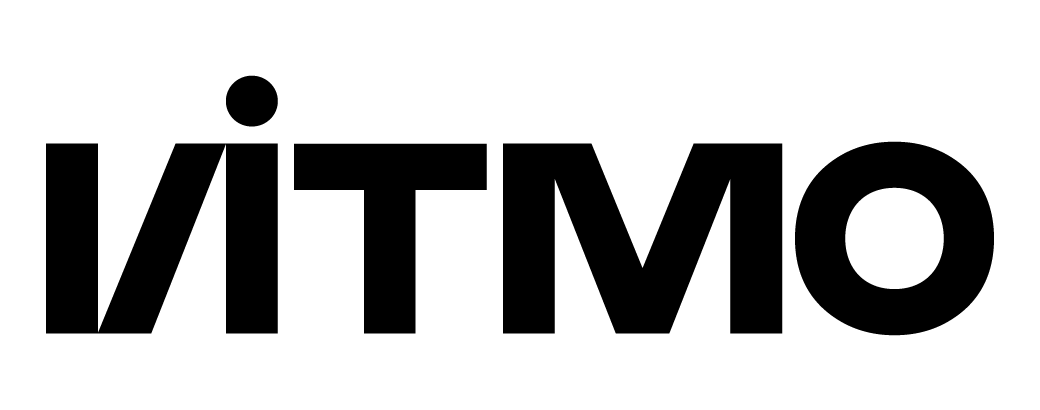
\includegraphics[width=0.26\textwidth]{../common/itmo-logo.png}\\
		\vspace{2.4cm}
		\textbf{\Large Основы электротехники}\\[1.2cm]
		\textbf{\Large Домашнее задание №#1}\\[0.7cm]
		\textbf{\Large #2}\\[3cm]

		\textbf{\Large Группа \textcolor{red}{\textit{P#3}}}\\[0.2cm]
		\textbf{\Large Вариант \textcolor{red}{\textit{#4}}}\\[3cm]

		\begin{flushleft}
			\textbf{\large Выполнил: \textcolor{red}{\textit{#5}}}\\[0.5cm]
			\textbf{\large Дата сдачи: \textcolor{red}{#6}}\\[0.5cm]
			\textbf{\large Контрольный срок сдачи: \uline{#7}}\\[0.5cm]
			\textbf{\large Количество баллов: \uline{#8}}\\[2cm]
		\end{flushleft}
	\end{center}

	\vspace*{\fill}
	\begin{center}
		\textbf{\Large СПб -- 2024}
	\end{center}
	\vspace*{-1.8cm}
}

% % listing for programming code blocks
\lstset{
	language=C++,                 % Programming language
	basicstyle=\ttfamily\normalsize, % Adjust font size
	keywordstyle=\color{blue},    % Style for keywords
	stringstyle=\color{red},      % Style for strings
	commentstyle=\color{gray},   % Style for comments
	morecomment=[l][\color{magenta}]{\#}, % Special comment style
	breaklines=true,              % Line breaking in long lines
	numbers=left,                 % Line numbering on the left
	numberstyle=\tiny\color{gray},% Style for line numbers
	frame=single,                 % Code frame
	showstringspaces=false        % Don't show spaces in strings
}

% % tikz styles for flowcharts
\tikzset{
	startstop/.style={
			rectangle,
			rounded corners,
			minimum width=3cm,
			minimum height=1cm,
			text centered,
			draw=black,
			fill=red!30
		},
	io/.style={
			trapezium,
			trapezium left angle=70,
			trapezium right angle=110,
			minimum width=3cm,
			minimum height=1cm,
			text centered,
			draw=black,
			fill=blue!30
		},
	process/.style={
			rectangle,
			minimum width=3cm,
			minimum height=1cm,
			text centered,
			draw=black,
			fill=orange!30
		},
	decision/.style={
			diamond,
			aspect=2,
			minimum width=3cm,
			text centered,
			draw=black,
			fill=green!30
		},
	arrow/.style={
			thick,
			->,
			>=stealth
		},
	prep/.style={
			chamfered rectangle,
			chamfered rectangle xsep=2cm,
			draw,
			thick,
			minimum width=5cm,
			minimum height=1cm,
			text centered,
			text width=2.5cm,
			font=\small,
			fill=yellow!30
		},
}


\begin{document}

% Title page
% old basic group uir title
\begin{center}
	\vspace{1cm}
	\large{Университет ИТМО}\\
	\large{Факультет программной инженерии и компьютерной техники}\\
	\vspace{4cm}
	\Large{\textbf{Учебно-исследовательская работа №1 (УИР 1)\\}}
	\vspace{0.3cm}
	\large{\textbf{<<Кодирование данных в телекоммуникационных системах>>\\}}
	\vspace{-0.3cm}
	\begin{center}
		\large{по дисциплине <<Телекоммуникационные системы>>}
	\end{center}
	\vspace{3cm}
\end{center}
\normalsize{
	\begin{flushright}
		Выполнил:
		\par
		Студент 3 курса группы P3331
		\par
		Дворкин Борис Александрович
		\par
		\textbf{Вариант: ДвБА}
		\par
		\vspace{1cm}
		Преподаватель:
		\par
		Алиеф Тауфик Измайлович
		\par
		\noindent Отчёт принят «\underline{\hspace{0.7cm}}» \underline{\hspace{1.3cm}} 2024 г.\\
		Оценка: \underline{\hspace{2cm}}
	\end{flushright}
}\\
\vspace{6cm}
\begin{center} г. Санкт-Петербург
	\par
	2024 г.
\end{center}
\thispagestyle{empty}
\thispagestyle{empty}


% -------------------------------

\newpage
\pagestyle{plain}
\setcounter{page}{1} % Enable text numbering

% -------------------------------

% autogenerated table of contents
\linespread{0.9}
\tableofcontents
\linespread{1}

% -------------------------------

\newpage
\section*{Цель работы}
\addcontentsline{toc}{section}{Цель работы}
Изучение методов \textit{физического} и \textit{логического} кодирования, используемых в цифровых сетях передачи данных.


% -------------------------------

\section{Формирование сообщения}
\begin{enumerate*}
\item ФИО: Дворкин Борис Александрович

\item Исходное сообщение: \textbf{ДвБА}

\item Сообщение состоит из 4 символов: Д, в, Б, А.

\begin{center}
	\begin{tabular}{|c|c|c|}
		\hline
		\textbf{Символ} & \textbf{В шестнадцатеричном коде} & \textbf{В двоичном коде} \\
		\hline
		Д               & C4                                & 1100\ 0100               \\
		в               & E2                                & 1110\ 0010               \\
		Б               & C1                                & 1100\ 0001               \\
		А               & C0                                & 1100\ 0000               \\
		\hline
	\end{tabular}
\end{center}

\item Итоговое сообщение в шестнадцатеричном коде:
\[
	\textbf{C4 E2 C1 C0}
\]

\item Итоговое сообщение в двоичном коде:
\[
	\textbf{1100 0100 1110 0010 1100 0001 1100 0000}
\]

\item Длина итогового сообщения: \textbf{4 байт (32 бит)}
\end{enumerate}


% -------------------------------

\section{Физическое кодирование}
\subsection{Потенциальный код без возврата к нулю (NRZ)}
Для определения верхней границы частот необходимо найти наиболее высокочастотную составляющую спектра в передаваемом сообщении, которая в NRZ образуется при передаче чередующихся значений 0 и 1, при этом период гармонического сигнала (синусоиды), используемого для передачи прямоугольных сигналов 0 и 1, будет равен удвоенной длительности битового интервала $\tau: T = 2\tau$, где $\tau$ определяется как величина, образная значению пропускной способности канала $C: \tau = \frac{1}{C}$. Отсюда верхняя граница частот будет равна \[f_{\text{в}} = \frac{1}{T} = \frac{C}{2}\]

То есть, при пропускной способности канала связи $C = 10 \, \text{Мбит/с}$ частота основной гармоники равна $f_{\text{в}} = \frac{10 \cdot 10^3}{2} = 5 \, \text{МГц}$, а битовый интервал $\tau = 100 \, \text{нс}$.

В общем случае, при кодировании любого сообщения с помощью метода NRZ наибольшая (верхняя) частота достигается при передаче чередующихся значений 0 и 1, а наименьшая (нижняя) - при передаче длинных (в пределе - бесконечных) последовательностей нулей и единиц, что делает нижнюю границу частот близкой и в пределе равной нулю: $f_{\text{н}} = 0$. Следовательно, в предельном случае спектр: $S = f_{\text{в}} - f_{\text{н}} = f_{\text{в}} = \frac{C}{2}$.

С другой стороны, при передаче конкретного сообщения нижняя частота всегда больше нуля и зависит от максимальной длины последовательностей нулей или единиц. В этом случае для расчёта нижней границы чапстот необходимо в коде передаваемого сообщения найти \textit{наиболее длинную последовательность 1 или 0}. В исходном сообщении, закодированном по методу NRZ, представленному на рисунке 1, низкочастотная составляющая образуется при передаче 6 последовательных нулей. Период синусоидального сигнала при передаче таких последовательностей равен 12 битовым интервалам и нижняя граница частот соответственно будет равна: $f_{\text{н}} = \frac{1}{12\tau} = \frac{C}{12}$. Тогда \textbf{спектр} при передаче данного сообщения кодом NRZ равен
\[
	S =  f_{\text{в}} - f_{\text{н}} = \frac{C}{2} - \frac{C}{12} = \frac{5C}{12} = 4.167 \, \text{МГц}
\]

Среднее значение частоты передаваемого сообщения находится в интервале $(f_{\text{н}};f_{\text{в}})$ и показывает, какие частоты (низкие или высокие) превалируют в спектре передаваемого сигнала.

Для оценки среднего значения частоты передаваемого сообщения можно для каждого битового интервала определить соответствующую частоту сигнала, просуммировать их и разделить на количество битовых интервалов. В нашем случае: частота основной гармоники $f_0 = \frac{C}{2}$ соответствует трём битовым интервалам, частота вдвое меньшая, т.е. $\frac{f_0}{2}$, соответствует также трём битовым интервалам, частота $\frac{f_0}{3}$ - четырём битовым интервалам, $\frac{f_0}{5}$ - одному битовому интервалу, и $\frac{f_0}{6}$ - одному битовому интервалу.

Тогда средняя частота рассматриваемого сообщения
\[
	f_{\text{ср}} = \left(3f_0+3\frac{f_0}{2}+4\frac{f_0}{3}+\frac{f_0}{5}+\frac{f_0}{6}\right)/ 12 = \frac{31f_0}{60} = \frac{31 \cdot 5}{60} \approx 2.583 \, \text{МГц}
\]

Поскольку середине спектра рассматриваемого сообщения соответствует частота
\[
	f_{1/2} = (f_{\text{н}} + f_{\text{в}}) /2 = \frac{\frac{C}{2} + \frac{C}{12}}{2} = \frac{7C}{24} = 2.917 \, \text{МГц}
\]
Можно констатировать, что в спектре сигнала \textit{незначительно превалируют низкие частоты}: $f_{\text{ср}} < f_{1/2}$.

Для качественной передачи двоичных сигналов по реальному каналу связи и возможности их распознавания на приёмной стороне с минимальным количеством ошибок, желательно на передающей стороне формировать сигналы, приближающиеся к прямоугольной форме. Однако, спектр таких сигналов оказывается слишком большим. Можно показать, что для качественного распознавания сигнала на приемной стороне при передаче чередующихся значений 0 и 1 достаточно сформировать сигнал, содержащий первые 4 гармоники (поскольку более высокочастотные гармоники оказывают незначительное влияние на результирующий сигнал) с частотами $f_0=\frac{C}{2}, f_1=3f_0, f_2=5f_0, f_3=7f_0$. В этом случае верхняя граница частот $f_{\text{в}}=7f_0$, а ширина спектра сигнала при передаче рассматриваемого сообщения соответственно будет равна $S = f_{\text{в}} - f_{\text{н}} = 7f_0-f_0/6=41f_0/6=34.167 \, \text{МГц}$.

Итак, при пропускной способности канала связи $C = 10 \, \text{Мбит/с}$ верхняя и нижняя границы частот в передаваемом сообщении равны соответственно $f_{\text{в}} = 5 \, \text{МГц}$ и $f_{\text{н}} = 0.833 \, \text{МГц}$, спектр сигнала $S = 4.167 \, \text{МГц}$, среднее значение частоты в спектре передаваемого сигнала $f_{\text{ср}} = 2.583 \, \text{МГц}$, полоса пропускания, необходимая для качественной передачи данного сообщения $F=35 \, \text{МГц}$.

Для определения верхней границы частот необходимо найти наиболее высокочастотную составляющую спектра в передаваемом сообщении, которая в NRZ образуется при передаче чередующихся значений 0 и 1, при этом период гармонического сигнала (синусоиды), используемого для передачи прямоугольных сигналов 0 и 1, будет равен удвоенной длительности битового интервала $\tau: T = 2\tau$, где $\tau$ определяется как величина, образная значению пропускной способности канала $C: \tau = \frac{1}{C}$. Отсюда верхняя граница частот будет равна \[f_{\text{в}} = \frac{1}{T} = \frac{C}{2}\]

То есть, при пропускной способности канала связи $C = 10 \, \text{Мбит/с}$ частота основной гармоники равна $f_{\text{в}} = \frac{10 \cdot 10^3}{2} = 5 \, \text{МГц}$, а битовый интервал $\tau = 100 \, \text{нс}$.

В общем случае, при кодировании любого сообщения с помощью метода NRZ наибольшая (верхняя) частота достигается при передаче чередующихся значений 0 и 1, а наименьшая (нижняя) - при передаче длинных (в пределе - бесконечных) последовательностей нулей и единиц, что делает нижнюю границу частот близкой и в пределе равной нулю: $f_{\text{н}} = 0$. Следовательно, в предельном случае спектр: $S = f_{\text{в}} - f_{\text{н}} = f_{\text{в}} = \frac{C}{2}$.

С другой стороны, при передаче конкретного сообщения нижняя частота всегда больше нуля и зависит от максимальной длины последовательностей нулей или единиц. В этом случае для расчёта нижней границы чапстот необходимо в коде передаваемого сообщения найти \textit{наиболее длинную последовательность 1 или 0}. В исходном сообщении, закодированном по методу NRZ, представленному на рисунке 1, низкочастотная составляющая образуется при передаче 6 последовательных нулей. Период синусоидального сигнала при передаче таких последовательностей равен 12 битовым интервалам и нижняя граница частот соответственно будет равна: $f_{\text{н}} = \frac{1}{12\tau} = \frac{C}{12}$. Тогда \textbf{спектр} при передаче данного сообщения кодом NRZ равен
\[
	S =  f_{\text{в}} - f_{\text{н}} = \frac{C}{2} - \frac{C}{12} = \frac{5C}{12} = 4.167 \, \text{МГц}
\]

Среднее значение частоты передаваемого сообщения находится в интервале $(f_{\text{н}};f_{\text{в}})$ и показывает, какие частоты (низкие или высокие) превалируют в спектре передаваемого сигнала.

Для оценки среднего значения частоты передаваемого сообщения можно для каждого битового интервала определить соответствующую частоту сигнала, просуммировать их и разделить на количество битовых интервалов. В нашем случае: частота основной гармоники $f_0 = \frac{C}{2}$ соответствует трём битовым интервалам, частота вдвое меньшая, т.е. $\frac{f_0}{2}$, соответствует также трём битовым интервалам, частота $\frac{f_0}{3}$ - четырём битовым интервалам, $\frac{f_0}{5}$ - одному битовому интервалу, и $\frac{f_0}{6}$ - одному битовому интервалу.

Тогда средняя частота рассматриваемого сообщения
\[
	f_{\text{ср}} = \left(3f_0+3\frac{f_0}{2}+4\frac{f_0}{3}+\frac{f_0}{5}+\frac{f_0}{6}\right)/ 12 = \frac{31f_0}{60} = \frac{31 \cdot 5}{60} \approx 2.583 \, \text{МГц}
\]

Поскольку середине спектра рассматриваемого сообщения соответствует частота
\[
	f_{1/2} = (f_{\text{н}} + f_{\text{в}}) /2 = \frac{\frac{C}{2} + \frac{C}{12}}{2} = \frac{7C}{24} = 2.917 \, \text{МГц}
\]
Можно констатировать, что в спектре сигнала \textit{незначительно превалируют низкие частоты}: $f_{\text{ср}} < f_{1/2}$.

Для качественной передачи двоичных сигналов по реальному каналу связи и возможности их распознавания на приёмной стороне с минимальным количеством ошибок, желательно на передающей стороне формировать сигналы, приближающиеся к прямоугольной форме. Однако, спектр таких сигналов оказывается слишком большим. Можно показать, что для качественного распознавания сигнала на приемной стороне при передаче чередующихся значений 0 и 1 достаточно сформировать сигнал, содержащий первые 4 гармоники (поскольку более высокочастотные гармоники оказывают незначительное влияние на результирующий сигнал) с частотами $f_0=\frac{C}{2}, f_1=3f_0, f_2=5f_0, f_3=7f_0$. В этом случае верхняя граница частот $f_{\text{в}}=7f_0$, а ширина спектра сигнала при передаче рассматриваемого сообщения соответственно будет равна $S = f_{\text{в}} - f_{\text{н}} = 7f_0-f_0/6=41f_0/6=34.167 \, \text{МГц}$.

Итак, при пропускной способности канала связи $C = 10 \, \text{Мбит/с}$ верхняя и нижняя границы частот в передаваемом сообщении равны соответственно $f_{\text{в}} = 5 \, \text{МГц}$ и $f_{\text{н}} = 0.833 \, \text{МГц}$, спектр сигнала $S = 4.167 \, \text{МГц}$, среднее значение частоты в спектре передаваемого сигнала $f_{\text{ср}} = 2.583 \, \text{МГц}$, полоса пропускания, необходимая для качественной передачи данного сообщения $F=35 \, \text{МГц}$.


% -----------------------------------------------------

\subsection{Биполярный импульсный код (RZ)}
\begin{figure}[H]
	\centering
	\begin{tikzpicture}[scale=0.48, very thick]
		\def\bits{1,1,0,0,0,1,0,0,1,1,1,0,0,0,1,0,1,1,0,0,0,0,0,1,1,1,0,0,0,0,0,0}

		\gdef\y{1}
		\foreach \b [count=\x from 0] in \bits {
			\draw[dashed, gray, thin] (\x+1,-1.5) -- (\x+1,2);
			\node at (\x+0.5, 2.5) {\small \b};
			\ifnum\b=1
				\ifnum\y=1
					\draw (\x,1) -- (\x+0.5,1) -- (\x+0.5,0) -- (\x+1,0);
					\xdef\y{0}
				\else
					\draw (\x,0) -- (\x,1) -- (\x+0.5,1) -- (\x+0.5,0) -- (\x+1,0);
					\xdef\y{0}
				\fi
			\else
				\draw (\x,0) -- (\x,-1) -- (\x+0.5,-1) -- (\x+0.5,0) -- (\x+1,0);
				\xdef\y{0}
			\fi
		}

		\draw[dashed, gray, thin] (0,0) -- (32,0);
		\draw[->] (0,-2) -- (0,2);

		\node[left] at (0,0) {0};
		\node[left] at (0,1) {1};
		\node[left] at (0,-1) {-1};
	\end{tikzpicture}
	\caption{RZ-кодирование исходного сообщения}
\end{figure}

\begin{figure}[H]
	\centering
	\begin{tikzpicture}[scale=0.48, very thick]
		\def\bits{1,1,0,0,0,1,0,0,1,1,1,0,0,0,1,0,1,1,0,0,0,0,0,1,1,1,0,0,0,0,0,0}

		\gdef\y{1}
		\foreach \b [count=\x from 0] in \bits {
			\draw[dashed, gray, thin] (\x+1,-1.5) -- (\x+1,2);
			\node at (\x+0.5, 2.5) {\small \b};
			\ifnum\b=1
				\ifnum\y=1
					\draw (\x,1) -- (\x+0.5,1) -- (\x+0.5,0) -- (\x+1,0);
					\xdef\y{0}
				\else
					\draw (\x,0) -- (\x,1) -- (\x+0.5,1) -- (\x+0.5,0) -- (\x+1,0);
					\xdef\y{0}
				\fi
			\else
				\draw (\x,0) -- (\x,-1) -- (\x+0.5,-1) -- (\x+0.5,0) -- (\x+1,0);
				\xdef\y{0}
			\fi
		}

		\draw[dashed, gray, thin] (0,0) -- (32,0);
		\draw[->] (0,-2) -- (0,2);

		\node[left] at (0,0) {0};
		\node[left] at (0,1) {1};
		\node[left] at (0,-1) {-1};
	\end{tikzpicture}
	\caption{RZ-кодирование исходного сообщения}
\end{figure}


% -----------------------------------------------------

\subsection{Потенциальный код с инверсий при 1 (NRZI)}
\begin{figure}[H]
	\centering
	\begin{tikzpicture}[scale=0.45, very thick]
		\def\bits{1,1,0,0,0,1,0,0,1,1,1,0,0,0,1,0,1,1,0,0,0,0,0,1,1,1,0,0,0,0,0,0}

		\gdef\y{0}
		\foreach \b [count=\x from 0] in \bits {
			\draw[dashed, gray, thin] (\x+1,-1) -- (\x+1,2);
			\node at (\x+0.5, 2.5) {\small \b};
			\ifnum\b=1
				\ifnum\y=1
					\draw (\x,1) -- (\x,0) -- (\x+1,0);
					\xdef\y{0}
				\else
					\draw (\x,0) -- (\x,1) -- (\x+1,1);
					\xdef\y{1}
				\fi
			\else
				\draw (\x,\y) -- (\x+1,\y);
			\fi
		}

		\draw[dashed, gray, thin] (0,0) -- (32,0);
		\draw[->] (0,-1.5) -- (0,2);

		\node[left] at (0,0) {0};
		\node[left] at (0,1) {1};
	\end{tikzpicture}
	\caption{NRZI-кодирование исходного сообщения}
\end{figure}

\begin{figure}[H]
	\centering
	\begin{tikzpicture}[scale=0.45, very thick]
		\def\bits{1,1,0,0,0,1,0,0,1,1,1,0,0,0,1,0,1,1,0,0,0,0,0,1,1,1,0,0,0,0,0,0}

		\gdef\y{0}
		\foreach \b [count=\x from 0] in \bits {
			\draw[dashed, gray, thin] (\x+1,-1) -- (\x+1,2);
			\node at (\x+0.5, 2.5) {\small \b};
			\ifnum\b=1
				\ifnum\y=1
					\draw (\x,1) -- (\x,0) -- (\x+1,0);
					\xdef\y{0}
				\else
					\draw (\x,0) -- (\x,1) -- (\x+1,1);
					\xdef\y{1}
				\fi
			\else
				\draw (\x,\y) -- (\x+1,\y);
			\fi
		}

		\draw[dashed, gray, thin] (0,0) -- (32,0);
		\draw[->] (0,-1.5) -- (0,2);

		\node[left] at (0,0) {0};
		\node[left] at (0,1) {1};
	\end{tikzpicture}
	\caption{NRZI-кодирование исходного сообщения}
\end{figure}


% -----------------------------------------------------

\subsection{Манчестерский код}
\begin{figure}[H]
	\centering
	\begin{tikzpicture}[scale=0.48, very thick]
		\def\bits{1,1,0,0,0,1,0,0,1,1,1,0,0,0,1,0,1,1,0,0,0,0,0,1,1,1,0,0,0,0,0,0}

		\gdef\y{1}
		\foreach \b [count=\x from 0] in \bits {
			\draw[dashed, gray, thin] (\x+1,-1) -- (\x+1,2);
			\node at (\x+0.5, 2.5) {\small \b};
			\ifnum\b=1
				\ifnum\y=1
					\draw (\x,1) -- (\x+0.5,1) -- (\x+0.5,0) -- (\x+1,0);
					\xdef\y{0}
				\else
					\draw (\x,0) -- (\x,1) -- (\x+0.5,1) -- (\x+0.5,0) -- (\x+1,0);
					\xdef\y{0}
				\fi
			\else
				\ifnum\y=1
					\draw (\x,1) -- (\x,0) -- (\x+0.5,0) -- (\x+0.5,1) -- (\x+1,1);
					\xdef\y{1}
				\else
					\draw (\x,0) -- (\x+0.5,0) -- (\x+0.5,1) -- (\x+1,1);
					\xdef\y{1}
				\fi
			\fi
		}

		\draw[dashed, gray, thin] (0,0) -- (32,0);
		\draw[->] (0,-1.5) -- (0,2);

		\node[left] at (0,0) {0};
		\node[left] at (0,1) {1};
	\end{tikzpicture}
	\caption{Манчестерское кодирование исходного сообщения}
\end{figure}

\begin{figure}[H]
	\centering
	\begin{tikzpicture}[scale=0.48, very thick]
		\def\bits{1,1,0,0,0,1,0,0,1,1,1,0,0,0,1,0,1,1,0,0,0,0,0,1,1,1,0,0,0,0,0,0}

		\gdef\y{1}
		\foreach \b [count=\x from 0] in \bits {
			\draw[dashed, gray, thin] (\x+1,-1) -- (\x+1,2);
			\node at (\x+0.5, 2.5) {\small \b};
			\ifnum\b=1
				\ifnum\y=1
					\draw (\x,1) -- (\x+0.5,1) -- (\x+0.5,0) -- (\x+1,0);
					\xdef\y{0}
				\else
					\draw (\x,0) -- (\x,1) -- (\x+0.5,1) -- (\x+0.5,0) -- (\x+1,0);
					\xdef\y{0}
				\fi
			\else
				\ifnum\y=1
					\draw (\x,1) -- (\x,0) -- (\x+0.5,0) -- (\x+0.5,1) -- (\x+1,1);
					\xdef\y{1}
				\else
					\draw (\x,0) -- (\x+0.5,0) -- (\x+0.5,1) -- (\x+1,1);
					\xdef\y{1}
				\fi
			\fi
		}

		\draw[dashed, gray, thin] (0,0) -- (32,0);
		\draw[->] (0,-1.5) -- (0,2);

		\node[left] at (0,0) {0};
		\node[left] at (0,1) {1};
	\end{tikzpicture}
	\caption{Манчестерское кодирование исходного сообщения}
\end{figure}


% -----------------------------------------------------

\subsection{Дифференциальный манчестерский код}
\begin{figure}[H]
	\centering
	\begin{tikzpicture}[scale=0.48, very thick]
		\def\bits{1,1,0,0,0,1,0,0,1,1,1,0,0,0,1,0,1,1,0,0,0,0,0,1,1,1,0,0,0,0,0,0}

		\gdef\y{1}
		\foreach \b [count=\x from 0] in \bits {
			\draw[dashed, gray, thin] (\x+1,-1) -- (\x+1,2);
			\node at (\x+0.5, 2.5) {\small \b};
			\ifnum\b=0
				\ifnum\y=1
					\draw (\x,1) -- (\x,0) -- (\x+0.5,0) -- (\x+0.5,1) -- (\x+1,1);
					\xdef\y{1}
				\else
					\draw (\x,0) -- (\x,1) -- (\x+0.5,1) -- (\x+0.5,0) -- (\x+1,0);
					\xdef\y{0}
				\fi
			\else
				\ifnum\y=1
					\draw (\x,1) -- (\x+0.5,1) -- (\x+0.5,0) -- (\x+1,0);
					\xdef\y{0}
				\else
					\draw (\x,0) -- (\x+0.5,0) -- (\x+0.5,1) -- (\x+1,1);
					\xdef\y{1}
				\fi
			\fi
		}

		\draw[dashed, gray, thin] (0,0) -- (32,0);
		\draw[->] (0,-1.5) -- (0,2);

		\node[left] at (0,0) {0};
		\node[left] at (0,1) {1};
	\end{tikzpicture}
	\caption{Манчестерское дифференциальное кодирование исходного сообщения}
\end{figure}

\begin{figure}[H]
	\centering
	\begin{tikzpicture}[scale=0.48, very thick]
		\def\bits{1,1,0,0,0,1,0,0,1,1,1,0,0,0,1,0,1,1,0,0,0,0,0,1,1,1,0,0,0,0,0,0}

		\gdef\y{1}
		\foreach \b [count=\x from 0] in \bits {
			\draw[dashed, gray, thin] (\x+1,-1) -- (\x+1,2);
			\node at (\x+0.5, 2.5) {\small \b};
			\ifnum\b=0
				\ifnum\y=1
					\draw (\x,1) -- (\x,0) -- (\x+0.5,0) -- (\x+0.5,1) -- (\x+1,1);
					\xdef\y{1}
				\else
					\draw (\x,0) -- (\x,1) -- (\x+0.5,1) -- (\x+0.5,0) -- (\x+1,0);
					\xdef\y{0}
				\fi
			\else
				\ifnum\y=1
					\draw (\x,1) -- (\x+0.5,1) -- (\x+0.5,0) -- (\x+1,0);
					\xdef\y{0}
				\else
					\draw (\x,0) -- (\x+0.5,0) -- (\x+0.5,1) -- (\x+1,1);
					\xdef\y{1}
				\fi
			\fi
		}

		\draw[dashed, gray, thin] (0,0) -- (32,0);
		\draw[->] (0,-1.5) -- (0,2);

		\node[left] at (0,0) {0};
		\node[left] at (0,1) {1};
	\end{tikzpicture}
	\caption{Манчестерское дифференциальное кодирование исходного сообщения}
\end{figure}


% -----------------------------------------------------

\subsection{PAM-5}
\begin{figure}[H]
	\centering
	\begin{tikzpicture}[scale=0.48, very thick]
		\def\bits{1,1,0,0,0,1,0,0,1,1,1,0,0,0,1,0,1,1,0,0,0,0,0,1,1,1,0,0,0,0,0,0}
		\def\bbits{11,00,01,00,11,10,00,10,11,00,00,01,11,00,00,00}

		\gdef\y{2}
		\foreach \b [count=\x from 0] in \bbits {
			\ifnum\b=11
				\draw (\x*2,\y) -- (\x*2,2) -- (\x*2+2,2);
				\xdef\y{2}
			\fi

			\ifnum\b=10
				\draw (\x*2,\y) -- (\x*2,1) -- (\x*2+2,1);
				\xdef\y{1}
			\fi

			\ifnum\b=01
				\draw (\x*2,\y) -- (\x*2,-1) -- (\x*2+2,-1);
				\xdef\y{-1}
			\fi

			\ifnum\b=00
				\draw (\x*2,\y) -- (\x*2,-2) -- (\x*2+2,-2);
				\xdef\y{-2}
			\fi
		}

		\foreach \b [count=\x from 0] in \bits {
			\draw[dashed, gray, thin] (\x+1,-3) -- (\x+1,3);
			\node at (\x+0.5, 3.5) {\small \b};
		}

		\draw[dashed, gray, thin] (0,0) -- (32,0);
		\draw[->] (0,-3) -- (0,3);

		\node[left] at (0,2) {11};
		\node[left] at (0,1) {10};
		\node[left] at (0,0) {};
		\node[left] at (0,-1) {01};
		\node[left] at (0,-2) {00};
	\end{tikzpicture}
	\caption{PAM-5-кодирование исходного сообщения}
\end{figure}

\begin{figure}[H]
	\centering
	\begin{tikzpicture}[scale=0.48, very thick]
		\def\bits{1,1,0,0,0,1,0,0,1,1,1,0,0,0,1,0,1,1,0,0,0,0,0,1,1,1,0,0,0,0,0,0}
		\def\bbits{11,00,01,00,11,10,00,10,11,00,00,01,11,00,00,00}

		\gdef\y{2}
		\foreach \b [count=\x from 0] in \bbits {
			\ifnum\b=11
				\draw (\x*2,\y) -- (\x*2,2) -- (\x*2+2,2);
				\xdef\y{2}
			\fi

			\ifnum\b=10
				\draw (\x*2,\y) -- (\x*2,1) -- (\x*2+2,1);
				\xdef\y{1}
			\fi

			\ifnum\b=01
				\draw (\x*2,\y) -- (\x*2,-1) -- (\x*2+2,-1);
				\xdef\y{-1}
			\fi

			\ifnum\b=00
				\draw (\x*2,\y) -- (\x*2,-2) -- (\x*2+2,-2);
				\xdef\y{-2}
			\fi
		}

		\foreach \b [count=\x from 0] in \bits {
			\draw[dashed, gray, thin] (\x+1,-3) -- (\x+1,3);
			\node at (\x+0.5, 3.5) {\small \b};
		}

		\draw[dashed, gray, thin] (0,0) -- (32,0);
		\draw[->] (0,-3) -- (0,3);

		\node[left] at (0,2) {11};
		\node[left] at (0,1) {10};
		\node[left] at (0,0) {};
		\node[left] at (0,-1) {01};
		\node[left] at (0,-2) {00};
	\end{tikzpicture}
	\caption{PAM-5-кодирование исходного сообщения}
\end{figure}



% -------------------------------

\section{Логическое кодирование}
\subsection{Избыточное кодирование методом 4B/5B}

\item Исходное сообщение в двоичном коде:
\[
	\textbf{1100 0100 1110 0010 1100 0001 1100 0000}
\]

\item Логическое кодирование методом 4B/5B:
\[
	\begin{array}{l l}
		\text{1100} & \rightarrow \text{11010} \\
		\text{0100} & \rightarrow \text{01010} \\
		\text{1110} & \rightarrow \text{11100} \\
		\text{0010} & \rightarrow \text{10100} \\
		\text{1100} & \rightarrow \text{11010} \\
		\text{0001} & \rightarrow \text{01001} \\
		\text{1100} & \rightarrow \text{11010} \\
		\text{0000} & \rightarrow \text{11110} \\
	\end{array}
\]

\item Результирующее сообщение после 4B/5B кодирования (в двоичном виде):
\[
	\textbf{11010 01010 11100 10100 11010 01001 11010 11110}
\]

\item Результирующее сообщение после 4B/5B кодирования (в шестнадцатеричном виде):
\[
	\textbf{1A 2A 1C 14 1A 09 1A 1E}
\]

\item Длина нового собщения: 40 бит (5 байт)
\item Избыточность кодирования:
\[
	\text{Избыточность} = \frac{40 - 32}{32} \times 100 = 25\%
\]

Я бы мог применить логическое кодирование к методам кодирования, выбранным на втором этапе в качестве наилучших, но это бы совершенно не имело смысла, так как суть логического кодирования в том, чтобы обеспечить синхронизацию и устранить постоянную составляющую, в чём оба Манчестерских кодирования совершенно не нуждаются. Поэтому, я выберу NRZI как третий лучший метод для кодирования, в виду простоты, дешевизны и крайне узкого спектра, что обеспечит высокую скорость передачи сообщения, а при логическом кодировании будет обеспечена надёжная синхронизация и устранение постоянной составляющей.

\subsection{Применим для кодирования NRZI}
\begin{figure}[H]
	\centering
	\begin{tikzpicture}[scale=0.41, very thick]
		\def\bits{1,1,0,1,0,0,1,0,1,0,1,1,1,0,0,1,0,1,0,0,1,1,0,1,0,0,1,0,0,1,1,1,0,1,0,1,1,1,1,0}

		\gdef\y{0}
		\foreach \b [count=\x from 0] in \bits {
			\draw[dashed, gray, thin] (\x+1,-1) -- (\x+1,2);
			\node at (\x+0.5, 2.5) {\small \b};
			\ifnum\b=1
				\ifnum\y=1
					\draw (\x,1) -- (\x,0) -- (\x+1,0);
					\xdef\y{0}
				\else
					\draw (\x,0) -- (\x,1) -- (\x+1,1);
					\xdef\y{1}
				\fi
			\else
				\draw (\x,\y) -- (\x+1,\y);
			\fi
		}

		\draw[dashed, gray, thin] (0,0) -- (32,0);
		\draw[->] (0,-1.5) -- (0,2);

		\node[left] at (0,0) {0};
		\node[left] at (0,1) {1};
	\end{tikzpicture}
	\caption{NRZI-кодирование избыточного сообщения}
\end{figure}

\begin{figure}[H]
	\centering
	\begin{tikzpicture}[scale=0.41, very thick]
		\def\bits{1,1,0,1,0,0,1,0,1,0,1,1,1,0,0,1,0,1,0,0,1,1,0,1,0,0,1,0,0,1,1,1,0,1,0,1,1,1,1,0}

		\gdef\y{0}
		\foreach \b [count=\x from 0] in \bits {
			\draw[dashed, gray, thin] (\x+1,-1) -- (\x+1,2);
			\node at (\x+0.5, 2.5) {\small \b};
			\ifnum\b=1
				\ifnum\y=1
					\draw (\x,1) -- (\x,0) -- (\x+1,0);
					\xdef\y{0}
				\else
					\draw (\x,0) -- (\x,1) -- (\x+1,1);
					\xdef\y{1}
				\fi
			\else
				\draw (\x,\y) -- (\x+1,\y);
			\fi
		}

		\draw[dashed, gray, thin] (0,0) -- (32,0);
		\draw[->] (0,-1.5) -- (0,2);

		\node[left] at (0,0) {0};
		\node[left] at (0,1) {1};
	\end{tikzpicture}
	\caption{NRZI-кодирование избыточного сообщения}
\end{figure}



% -------------------------------

\section{Скремблирование}
\subsection{Скремблирование исходного сообщения}
\begin{enumerate}
	\item \textbf{Выберем алгоритм преобразования:}
	      \[
		      B_i = A_i \oplus B_{i-3} \oplus B_{i-5} \quad (i = 1, 2, \ldots, 32)
	      \]

	\item \textbf{Исходное сообщение:}
	      \[
		      \textbf{1100\ 0100\ 1110\ 0010\ 1100\ 0001\ 1100\ 0000}
	      \]

	\item \textbf{Скремблированное сообщение:}
	      \[
		      \begin{array}{ll}
			      B_1 = A_1 = 1                                                         \\
			      B_2 = A_2 = 1                                                         \\
			      B_3 = A_3 = 0                                                         \\
			      B_4 = A_4 \oplus B_1 = 0 \oplus 1 = 1                                 \\
			      B_5 = A_5 \oplus B_2 = 0 \oplus 1 = 1                                 \\
			      B_6 = A_6 \oplus B_3 \oplus B_1 = 1 \oplus 0 \oplus 1 = 0             \\
			      B_7 = A_7 \oplus B_4 \oplus B_2 = 0 \oplus 1 \oplus 1 = 0             \\
			      B_8 = A_8 \oplus B_5 \oplus B_3 = 0 \oplus 1 \oplus 0 = 1             \\
			      B_9 = A_9 \oplus B_6 \oplus B_4 = 1 \oplus 0 \oplus 1 = 0             \\
			      B_{10} = A_{10} \oplus B_7 \oplus B_5 = 1 \oplus 0 \oplus 1 = 0       \\
			      B_{11} = A_{11} \oplus B_8 \oplus B_6 = 1 \oplus 1 \oplus 0 = 0       \\
			      B_{12} = A_{12} \oplus B_9 \oplus B_7 = 0 \oplus 0 \oplus 0 = 0       \\
			      B_{13} = A_{13} \oplus B_{10} \oplus B_8 = 0 \oplus 0 \oplus 1 = 1    \\
			      B_{14} = A_{14} \oplus B_{11} \oplus B_9 = 0 \oplus 0 \oplus 0 = 0    \\
			      B_{15} = A_{15} \oplus B_{12} \oplus B_{10} = 1 \oplus 0 \oplus 0 = 1 \\
			      B_{16} = A_{16} \oplus B_{13} \oplus B_{11} = 0 \oplus 1 \oplus 0 = 1 \\
			      B_{17} = A_{17} \oplus B_{14} \oplus B_{12} = 1 \oplus 0 \oplus 0 = 1 \\
			      B_{18} = A_{18} \oplus B_{15} \oplus B_{13} = 1 \oplus 1 \oplus 1 = 1 \\
			      B_{19} = A_{19} \oplus B_{16} \oplus B_{14} = 0 \oplus 1 \oplus 0 = 1 \\
			      B_{20} = A_{20} \oplus B_{17} \oplus B_{15} = 0 \oplus 1 \oplus 1 = 0 \\
			      B_{21} = A_{21} \oplus B_{18} \oplus B_{16} = 0 \oplus 1 \oplus 1 = 0 \\
			      B_{22} = A_{22} \oplus B_{19} \oplus B_{17} = 0 \oplus 1 \oplus 1 = 0 \\
			      B_{23} = A_{23} \oplus B_{20} \oplus B_{18} = 0 \oplus 0 \oplus 1 = 1 \\
			      B_{24} = A_{24} \oplus B_{21} \oplus B_{19} = 1 \oplus 0 \oplus 1 = 0 \\
			      B_{25} = A_{25} \oplus B_{22} \oplus B_{20} = 1 \oplus 0 \oplus 0 = 1 \\
			      B_{26} = A_{26} \oplus B_{23} \oplus B_{21} = 1 \oplus 1 \oplus 0 = 0 \\
			      B_{27} = A_{27} \oplus B_{24} \oplus B_{22} = 0 \oplus 0 \oplus 0 = 0 \\
			      B_{28} = A_{28} \oplus B_{25} \oplus B_{23} = 0 \oplus 1 \oplus 1 = 0 \\
			      B_{29} = A_{29} \oplus B_{26} \oplus B_{24} = 0 \oplus 0 \oplus 0 = 0 \\
			      B_{30} = A_{30} \oplus B_{27} \oplus B_{25} = 0 \oplus 0 \oplus 1 = 1 \\
			      B_{31} = A_{31} \oplus B_{28} \oplus B_{26} = 0 \oplus 0 \oplus 0 = 0 \\
			      B_{32} = A_{32} \oplus B_{29} \oplus B_{27} = 0 \oplus 0 \oplus 0 = 0 \\
		      \end{array}
	      \]

	\item Получили новое сообщение, в котором всё равно присутствует достаточно длинная последовательность из 4х нулей, но главное избавились от последовательностей из 6 и из 5 нулей в исходном сообщении, что существенно улучшит синхронизацию.

	\item \textbf{Результат скремблирования: (в двоичном виде)}
	      \[
		      \textbf{1101\ 1001\ 0000\ 1011\ 1110\ 0001\ 1000\ 0100}
	      \]

	\item \textbf{Результат скремблирования (в шестнадцатеричном виде):}
	      \[
		      \textbf{D9 0B E1 84}
	      \]
\end{enumerate}

По аналогичным причинам, что я описал в конце этапа избыточного кодирования, применю скремблированное сообщение для кодирования NRZI.
\subsection{Применим для кодирования NRZI}
Для определения верхней границы частот необходимо найти наиболее высокочастотную составляющую спектра в передаваемом сообщении, которая в NRZI образуется при передаче последовательных значений 0 и 1, при этом период гармонического сигнала (синусоиды), используемого для передачи прямоугольных сигналов 0 и 1, будет равен удвоенной длительности битового интервала $\tau: T = 2\tau$, где $\tau$ определяется как величина, образная значению пропускной способности канала $C: \tau = \frac{1}{C}$. Отсюда верхняя граница частот будет равна \[f_{\text{в}} = \frac{1}{T} = \frac{C}{2}\]

В общем случае, при кодировании любого сообщения с помощью метода NRZI наибольшая (верхняя) частота достигается при передаче последовательных значений 0 и 1, а наименьшая (нижняя) - при передаче длинных (в пределе - бесконечных) последовательностей нулей, что делает нижнюю границу частот близкой и в пределе равной нулю: $f_{\text{н}} = 0$. Следовательно, в предельном случае спектр: $S = f_{\text{в}} - f_{\text{н}} = f_{\text{в}} = \frac{C}{2}$.

С другой стороны, при передаче конкретного сообщения нижняя частота всегда больше нуля и зависит от максимальной длины последовательностей нулей. В этом случае для расчёта нижней границы чапстот необходимо в коде передаваемого сообщения найти \textit{наиболее длинную последовательность нулей}. В исходном сообщении, закодированном по методу NRZI, представленному на рисунке 1, низкочастотная составляющая образуется при передаче единицы и 4 последовательных нулей. Период синусоидального сигнала при передаче таких последовательностей равен 10 битовым интервалам и нижняя граница частот соответственно будет равна: $f_{\text{н}} = \frac{1}{10\tau} = \frac{C}{10}$. Тогда \textbf{спектр} при передаче данного сообщения кодом NRZI равен
\[
	S =  f_{\text{в}} - f_{\text{н}} = \frac{C}{2} - \frac{C}{10} = \frac{2C}{5} = 4 \, \text{МГц}
\]

То есть, при пропускной способности канала связи $C = 10 \, \text{Мбит/с}$ частота основной гармоники равна $f_{\text{в}} = \frac{10 \cdot 10^3}{2} = 5 \, \text{МГц}$, битовый интервал $\tau = 100 \, \text{нс}$, а нижняя частота гармоники $f_{\text{н}} = 1 \, \text{МГц}$.

Среднее значение частоты передаваемого сообщения находится в интервале $(f_{\text{н}};f_{\text{в}})$ и показывает, какие частоты (низкие или высокие) превалируют в спектре передаваемого сигнала.

Для оценки среднего значения частоты передаваемого сообщения можно для каждого битового интервала определить соответствующую частоту сигнала, просуммировать их и разделить на количество битовых интервалов. В нашем случае: частота основной гармоники $f_0 = \frac{C}{2}$ соответствует 7 битовым интервалам, частота вдвое меньшая, т.е. $\frac{f_0}{2}$, соответствует 2 битовым интервалам, частота $\frac{f_0}{3}$ - также 2 битовым интервалам и частота $\frac{f_0}{4}$ - 3 битовым интервалам.

Тогда средняя частота рассматриваемого сообщения
\[
	f_{\text{ср}} = \left(7f_0+2\frac{f_0}{2}+2\frac{f_0}{3}+3\frac{f_0}{4}\right)/ 14 = \frac{113f_0}{168} = \frac{113 \cdot 5}{168} \approx 3.363 \, \text{МГц}
\]

Поскольку середине спектра рассматриваемого сообщения соответствует частота
\[
	f_{1/2} = (f_{\text{н}} + f_{\text{в}}) /2 = 3.334 \, \text{МГц}
\]
Можно констатировать, что в спектре сигнала практически идеальный баланс низких и высоких частот: $f_{\text{ср}} \approx f_{1/2}$.

Для качественной передачи двоичных сигналов по реальному каналу связи и возможности их распознавания на приёмной стороне с минимальным количеством ошибок, желательно на передающей стороне формировать сигналы, приближающиеся к прямоугольной форме. Однако, спектр таких сигналов оказывается слишком большим. Можно показать, что для качественного распознавания сигнала на приемной стороне при передаче чередующихся значений 0 и 1 достаточно сформировать сигнал, содержащий первые 4 гармоники (поскольку более высокочастотные гармоники оказывают незначительное влияние на результирующий сигнал) с частотами $f_0=\frac{C}{2}, f_1=3f_0, f_2=5f_0, f_3=7f_0$. В этом случае верхняя граница частот $f_{\text{в}}=7f_0$, а ширина спектра сигнала при передаче рассматриваемого сообщения соответственно будет равна $S = f_{\text{в}} - f_{\text{н}} = 7f_0-f_0/4=27f_0/4=33.75 \, \text{МГц}$. Полоса пропускания F, необходимая для качественной передачи данного сообщения, должна быть не меньше спектра S, например, $F = 34 \, \text{МГц}$.

Итак, при пропускной способности канала связи $C = 10 \, \text{Мбит/с}$ верхняя и нижняя границы частот в передаваемом сообщении равны соответственно $f_{\text{в}} = 5 \, \text{МГц}$ и $f_{\text{н}} = 1 \, \text{МГц}$, спектр сигнала $S = 4 \, \text{МГц}$, среднее значение частоты в спектре передаваемого сигнала $f_{\text{ср}} = 3.363 \, \text{МГц}$, полоса пропускания, необходимая для качественной передачи данного сообщения $F=34 \, \text{МГц}$.

Для определения верхней границы частот необходимо найти наиболее высокочастотную составляющую спектра в передаваемом сообщении, которая в NRZI образуется при передаче последовательных значений 0 и 1, при этом период гармонического сигнала (синусоиды), используемого для передачи прямоугольных сигналов 0 и 1, будет равен удвоенной длительности битового интервала $\tau: T = 2\tau$, где $\tau$ определяется как величина, образная значению пропускной способности канала $C: \tau = \frac{1}{C}$. Отсюда верхняя граница частот будет равна \[f_{\text{в}} = \frac{1}{T} = \frac{C}{2}\]

В общем случае, при кодировании любого сообщения с помощью метода NRZI наибольшая (верхняя) частота достигается при передаче последовательных значений 0 и 1, а наименьшая (нижняя) - при передаче длинных (в пределе - бесконечных) последовательностей нулей, что делает нижнюю границу частот близкой и в пределе равной нулю: $f_{\text{н}} = 0$. Следовательно, в предельном случае спектр: $S = f_{\text{в}} - f_{\text{н}} = f_{\text{в}} = \frac{C}{2}$.

С другой стороны, при передаче конкретного сообщения нижняя частота всегда больше нуля и зависит от максимальной длины последовательностей нулей. В этом случае для расчёта нижней границы чапстот необходимо в коде передаваемого сообщения найти \textit{наиболее длинную последовательность нулей}. В исходном сообщении, закодированном по методу NRZI, представленному на рисунке 1, низкочастотная составляющая образуется при передаче единицы и 4 последовательных нулей. Период синусоидального сигнала при передаче таких последовательностей равен 10 битовым интервалам и нижняя граница частот соответственно будет равна: $f_{\text{н}} = \frac{1}{10\tau} = \frac{C}{10}$. Тогда \textbf{спектр} при передаче данного сообщения кодом NRZI равен
\[
	S =  f_{\text{в}} - f_{\text{н}} = \frac{C}{2} - \frac{C}{10} = \frac{2C}{5} = 4 \, \text{МГц}
\]

То есть, при пропускной способности канала связи $C = 10 \, \text{Мбит/с}$ частота основной гармоники равна $f_{\text{в}} = \frac{10 \cdot 10^3}{2} = 5 \, \text{МГц}$, битовый интервал $\tau = 100 \, \text{нс}$, а нижняя частота гармоники $f_{\text{н}} = 1 \, \text{МГц}$.

Среднее значение частоты передаваемого сообщения находится в интервале $(f_{\text{н}};f_{\text{в}})$ и показывает, какие частоты (низкие или высокие) превалируют в спектре передаваемого сигнала.

Для оценки среднего значения частоты передаваемого сообщения можно для каждого битового интервала определить соответствующую частоту сигнала, просуммировать их и разделить на количество битовых интервалов. В нашем случае: частота основной гармоники $f_0 = \frac{C}{2}$ соответствует 7 битовым интервалам, частота вдвое меньшая, т.е. $\frac{f_0}{2}$, соответствует 2 битовым интервалам, частота $\frac{f_0}{3}$ - также 2 битовым интервалам и частота $\frac{f_0}{4}$ - 3 битовым интервалам.

Тогда средняя частота рассматриваемого сообщения
\[
	f_{\text{ср}} = \left(7f_0+2\frac{f_0}{2}+2\frac{f_0}{3}+3\frac{f_0}{4}\right)/ 14 = \frac{113f_0}{168} = \frac{113 \cdot 5}{168} \approx 3.363 \, \text{МГц}
\]

Поскольку середине спектра рассматриваемого сообщения соответствует частота
\[
	f_{1/2} = (f_{\text{н}} + f_{\text{в}}) /2 = 3.334 \, \text{МГц}
\]
Можно констатировать, что в спектре сигнала практически идеальный баланс низких и высоких частот: $f_{\text{ср}} \approx f_{1/2}$.

Для качественной передачи двоичных сигналов по реальному каналу связи и возможности их распознавания на приёмной стороне с минимальным количеством ошибок, желательно на передающей стороне формировать сигналы, приближающиеся к прямоугольной форме. Однако, спектр таких сигналов оказывается слишком большим. Можно показать, что для качественного распознавания сигнала на приемной стороне при передаче чередующихся значений 0 и 1 достаточно сформировать сигнал, содержащий первые 4 гармоники (поскольку более высокочастотные гармоники оказывают незначительное влияние на результирующий сигнал) с частотами $f_0=\frac{C}{2}, f_1=3f_0, f_2=5f_0, f_3=7f_0$. В этом случае верхняя граница частот $f_{\text{в}}=7f_0$, а ширина спектра сигнала при передаче рассматриваемого сообщения соответственно будет равна $S = f_{\text{в}} - f_{\text{н}} = 7f_0-f_0/4=27f_0/4=33.75 \, \text{МГц}$. Полоса пропускания F, необходимая для качественной передачи данного сообщения, должна быть не меньше спектра S, например, $F = 34 \, \text{МГц}$.

Итак, при пропускной способности канала связи $C = 10 \, \text{Мбит/с}$ верхняя и нижняя границы частот в передаваемом сообщении равны соответственно $f_{\text{в}} = 5 \, \text{МГц}$ и $f_{\text{н}} = 1 \, \text{МГц}$, спектр сигнала $S = 4 \, \text{МГц}$, среднее значение частоты в спектре передаваемого сигнала $f_{\text{ср}} = 3.363 \, \text{МГц}$, полоса пропускания, необходимая для качественной передачи данного сообщения $F=34 \, \text{МГц}$.



% -------------------------------

\section{Сравнительный анализ}
\begin{table}[H]
	\centering
	\scalebox{0.75}{
		\renewcommand{\arraystretch}{1.2}
		\begin{tabular}{|>{\centering\arraybackslash}m{3.8cm}|
			>{\centering\arraybackslash}m{4cm}|
			>{\centering\arraybackslash}m{3cm}|
			>{\centering\arraybackslash}m{3cm}|
			>{\centering\arraybackslash}m{3cm}|
			>{\centering\arraybackslash}m{3.5cm}|}
			\hline
			\textbf{Метод кодирования}                                                         & \textbf{Спектральные характеристики} & \textbf{Постоянная составляющая} & \textbf{Самосин- хронизация} & \textbf{Обнаруж. ошибок} & \textbf{Сложность реализации} \\
			\hline
			\textbf{Потенциальный код с инверсией при единице (NRZI)}                          &
			Малая ширина спектра ($0$--$\frac{C}{2}$), итоговый спектр $\frac{3C}{7}$          &
			Присутствует, но снижена по сравнению с NRZ                                        &
			Отсутствует, возможны проблемы при длинных последовательностях '0'                 &
			Отсутствует                                                                        &
			Низкая сложность реализации, два уровня потенциала $\implies$ низкая стоимость                                                                                                                                                                         \\
			\hline
			\textbf{Манчестерское кодирование (М2)}                                            &
			Большая ширина спектра ($0$--$C$), итоговый спектр $C$                             &
			Отсутствует                                                                        &
			Отличная, переход в середине каждого битового интервала обеспечивает синхронизацию &
			Отсутствует                                                                        &
			Средняя сложность реализации, два уровня потенциала $\implies$ умеренная стоимость                                                                                                                                                                     \\
			\hline
			\textbf{Дифф. манчестерское кодирование}                                           &
			Большая ширина спектра ($0$--$C$), итоговый спектр $C$                             &
			Отсутствует                                                                        &
			Отличная, устойчива к инверсии сигнала                                             &
			Отсутствует                                                                        &
			Высокая сложность реализации, два уровня потенциала $\implies$ умеренная стоимость                                                                                                                                                                     \\
			\hline
			\textbf{NRZI с 4B/5B кодированием}                                                 &
			Уменьшенный итоговый спектр: $\frac{C}{3}$                                         &
			Отсутствует (благодаря 4B/5B)                                                      &
			Улучшена, длинные последовательности '0' полностью устранены                       &
			Отсутствует                                                                        &
			Низкая сложность реализации, простое сопоставление битов таблицей кодировки                                                                                                                                                                            \\
			\hline
			\textbf{NRZI со скремблированием}                                                  &
			Меньше спектр, чем у изначального NRZI, но больше 4B/5B: $\frac{2C}{5}$            &
			Отсутствует (благодаря скремблированию)                                            &
			Улучшена, благодаря скремблированию, но остались длинные последовательности '0'    &
			Отсутствует                                                                        &
			Средняя сложность реализации, считать полином для каждого преобразования долго и муторно                                                                                                                                                               \\
			\hline
		\end{tabular}
	}
	\caption{Сравнение методов кодирования из этапов 2, 3 и 4}
\end{table}

\textbf{NRZI} снижает постоянную составляющую по сравнению с NRZ и сохраняет простоту реализации. Однако его эффективность сильно зависит от статистики передаваемых данных; при длинных последовательностях '0' возможны проблемы с синхронизацией, а постоянная составляющая всё ещё присутствует. Тем не менее, по сравнению с AMI, который является его прямым конкурентом, но не был рассмотрен в данном отчёте, NRZI имеет лишь два уровня потенциала, что делает его дешевле и предпочтительнее для использования.

С помощью методов логического кодирования можно существенно улучшить NRZI.

\textbf{NRZI с 4B/5B кодированием} устраняет постоянную составляющую и улучшает синхронизацию благодаря введению избыточности. Длинные последовательности нулей заменяются кодами без длительных последовательностей нулей, что повышает надёжность передачи. Спектр после 4B/5B кодирования стал $\frac{C}{3} = 3.333 \, \text{МГц}$, что на 0.7 МГц меньше, чем при скремблировании того же метода кодирования, что существенно повышает скорость передачи сообщения.

\textbf{NRZI со скремблированием} лишь частично устраняет длинные последовательности одинаковых битов, улучшая синхронизацию и также устраняя постоянную составляющую. При этом сохраняется узкая полоса пропускания, а сложность реализации существенно выше, чем у избыточного кодирования 4B/5B, а также спектр выше на 0.7 МГц.

\textbf{Манчестерское кодирование} обеспечивает отличную синхронизацию и не имеет постоянной составляющей, что повышает надёжность передачи. Однако в сравнении с NRZI с 4B/5B кодированием, мы получаем на 2/3 C меньший спектр, при этом не проигрывая в синхронизации и постоянной составляющей. Таким образом, Манчестерское кодирование получается сложнее NRZI с 4B/5B кодированием, и дороже в реализации, не имея перед ним преимуществ.

\textbf{Дифференциальное манчестерское кодирование} наследует преимущества манчестерского кодирования и дополнительно устойчиво к инверсии сигнала, что важно в шумных средах. Хотя высокая сложность реализации и широкий спектр являются его недостатками, NRZI с 4B/5B кодированием не имеет устойчивости к инверсии сигнала - оно имеет лишь частичную возможность обнаружения ошибок за счёт наличия запрещённых символов. Исходя из этого, если важно иметь устойчивость к инверсии сигнала и есть возможность пожертвовать спектром, а соответственно более низкой скорости передачи сообщения, то предпочтительнее будет выбрать Дифференциальное манчестерское кодирование.




% -------------------------------

\section{Выводы}
В результате применения логического кодирования и скремблирования к исходному сообщению при использовании метода NRZI удалось значительно улучшить характеристики сигнала по сравнению с исходным методом NRZI. Благодаря избыточному кодированию 4B/5B и скремблированию были устранены длинные последовательности нулей, что повысило надёжность синхронизации и устранило постоянную составляющую сигнала. При этом сохраняется узкая полоса пропускания и низкая сложность реализации, что делает эти методы эффективными для использования в системах с ограниченными ресурсами и требованиями к полосе пропускания.

По сравнению с манчестерскими методами кодирования, NRZI с логическим кодированием или скремблированием обеспечивает более эффективное использование полосы пропускания, так как требует меньшей ширины спектра. Однако манчестерское и дифференциальное манчестерское кодирование всё ещё превосходят по надёжности синхронизации и устойчивости к помехам, что делает их предпочтительными в системах, где эти факторы являются критически важными.

Таким образом, применение логических кодирований и скремблирования позволяет улучшить характеристики методов с низкой сложностью реализации, не имеющих надёжной синхронизации и обнаружения ошибок, приближая их по качеству к более сложным методам, таким как манчестерское кодирование. Выбор между этими методами должен основываться на конкретных требованиях системы передачи данных, включая допустимую полосу пропускания, сложность реализации и необходимость в надёжной синхронизации.


\end{document}
